\documentclass[12pt]{article}
\usepackage[utf8]{inputenc}
\usepackage{amsmath}
\usepackage{amssymb}
\usepackage{mathtools}
\usepackage{amsfonts}
\usepackage{lastpage}
\usepackage{tikz}
\usepackage{pdfpages}
\usepackage{gauss}
\usepackage{fancyvrb}
\usepackage{fancyhdr}
\usepackage{graphicx}
\pagestyle{fancy}
\fancyfoot[C]{\footnotesize Page \thepage\ of 3}
\DeclareGraphicsExtensions{.pdf,.png,.jpg}
\title{Elementær Talteori}
\author{Nikolaj Dybdahl Rathcke}
\chead{Nikolaj Dybdahl Rathcke (rfq695)}

\begin{document}
\section{1.3.1}
Lad sekvenserne være
\begin{align*}
x_1&=[1,0,-2,-6-14,-30,...] \\
x_2&=[1,1,1,1,...] \\
x_3&=[2,4,8,16,...]
\end{align*}
Dette kan bruges til at opstille ligningerne
\begin{align*}
1&=a+2b \\
0&=a+4b
\end{align*}
Hvoraf vi kan udregne de 2 konstanter ved at isolere $b$ i den anden ligning og sætte dette udtryk ind i den første for $b$ for at få $a$
\begin{align*}
0&=a+4b \\
b&=-\frac{a}{4} \\
1&=a+2(-\frac{a}{4}) \\
a&=2
\end{align*}
Og herefter udregne $b$
\begin{align*}
1&=2+2b \\
b&=-\frac{1}{2}
\end{align*}
Af dette kan vi opstille den første sekvens som en lineær kombination af de 2 andre sekvenser.
\begin{align*}
x_1=2x_{2}-\frac{1}{2}x_{3}
\end{align*}

\section{1.3.11}
\subsection{a}
Vi kan opstille det karakteristiske polynomium
$$\lambda^3-3\lambda^2+4=0$$
Hvor af rødderne kan udregnes\\
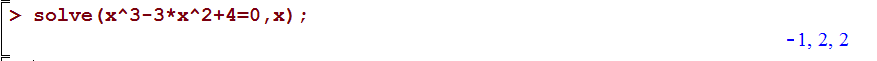
\includegraphics[width=\textwidth]{1}\\
og rodden $2$ har multiplicitet $2$, så $\lambda_1=-1$,$\lambda_2=2$ og $\lambda_3=2$.\\
Vi kan finde basis løsningerne til dette
\begin{align*}
x(-1)&=[\lambda_1^1,\lambda_1^2,\lambda_1^3,\lambda_1^4,...] \\
&=[-1,1,-1,1,...] \\
x(2)&=[\lambda_2^1,\lambda_2^2,\lambda_2^3,\lambda_2^4,...] \\
&=[2,4,8,16,...] \\
x'(2)&=[\frac{\partial}{\partial\lambda}\lambda_3^1,\frac{\partial}{\partial\lambda}\lambda_3^2,\frac{\partial}{\partial\lambda}\lambda_3^3,\frac{\partial}{\partial\lambda}\lambda_3^4,...] \\
&=[1\lambda_3^0,2\lambda_3^1,3\lambda_3^2,4\lambda_3^3,...] \\
&=[1,-2,3,-4,...]
\end{align*}
Altså har vi basis løsningerne
\begin{align*}
x_1&=[-1,1,-1,1,...] \\
x_2&=[2,4,8,16,...] \\
x_3&=[1,-2,3,-4,...]
\end{align*}

\subsection{b}
Vi ser at det er det karakteristiske polynomium
$$\lambda^2-2\lambda+3=0$$
Med rødderne\\
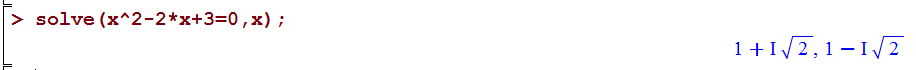
\includegraphics[width=\textwidth]{2}\\
hvor begge rødder er komplekse og har multiplicitet 1, så $\lambda_1=1+I\sqrt{2}$ og $\lambda_2=1-I\sqrt{2}$.\\
Vi kan så finde basis løsningerne ved brug af Maple.
\begin{align*}
x(1+I\sqrt{2})&=[\lambda_1^1,\lambda_1^2,\lambda_1^3,\lambda_1^4,...] \\
&=[1+I\sqrt{2},-1+2I\sqrt{2},-5+I\sqrt{2},-7-4I\sqrt{2},...] \\
x(1-I\sqrt{2})&=[\lambda_2^1,\lambda_2^2,\lambda_2^3,\lambda_2^4,...] \\
&=[1-I\sqrt{2},-1-2I\sqrt{2},-5-I\sqrt{2},-7+4I\sqrt{2},...] \\
\end{align*}
Og igen er basis løsningerne altså
\begin{align*}
x_1&=[1+I\sqrt{2},-1+2I\sqrt{2},-5+I\sqrt{2},-7-4I\sqrt{2},...] \\
x_2&=[1-I\sqrt{2},-1-2I\sqrt{2},-5-I\sqrt{2},-7+4I\sqrt{2},...] 
\end{align*}

\section{JH-3}


\end{document}
